\documentclass{article}

\usepackage{graphicx}
\usepackage{tikz}
\usepackage{tikzsymbols}
\usetikzlibrary{calc,patterns,shapes.geometric}
\pagestyle{empty}
\usepackage[margin=0pt]{geometry}
\geometry{papersize={14in,12in}}

\def\centerarc[#1](#2)(#3:#4:#5){\draw[#1] ($(#2)+({#5*cos(#3)},{#5*sin(#3)})$) arc (#3:#4:#5);}

\begin{document}
	\begin{figure}
		\centering
		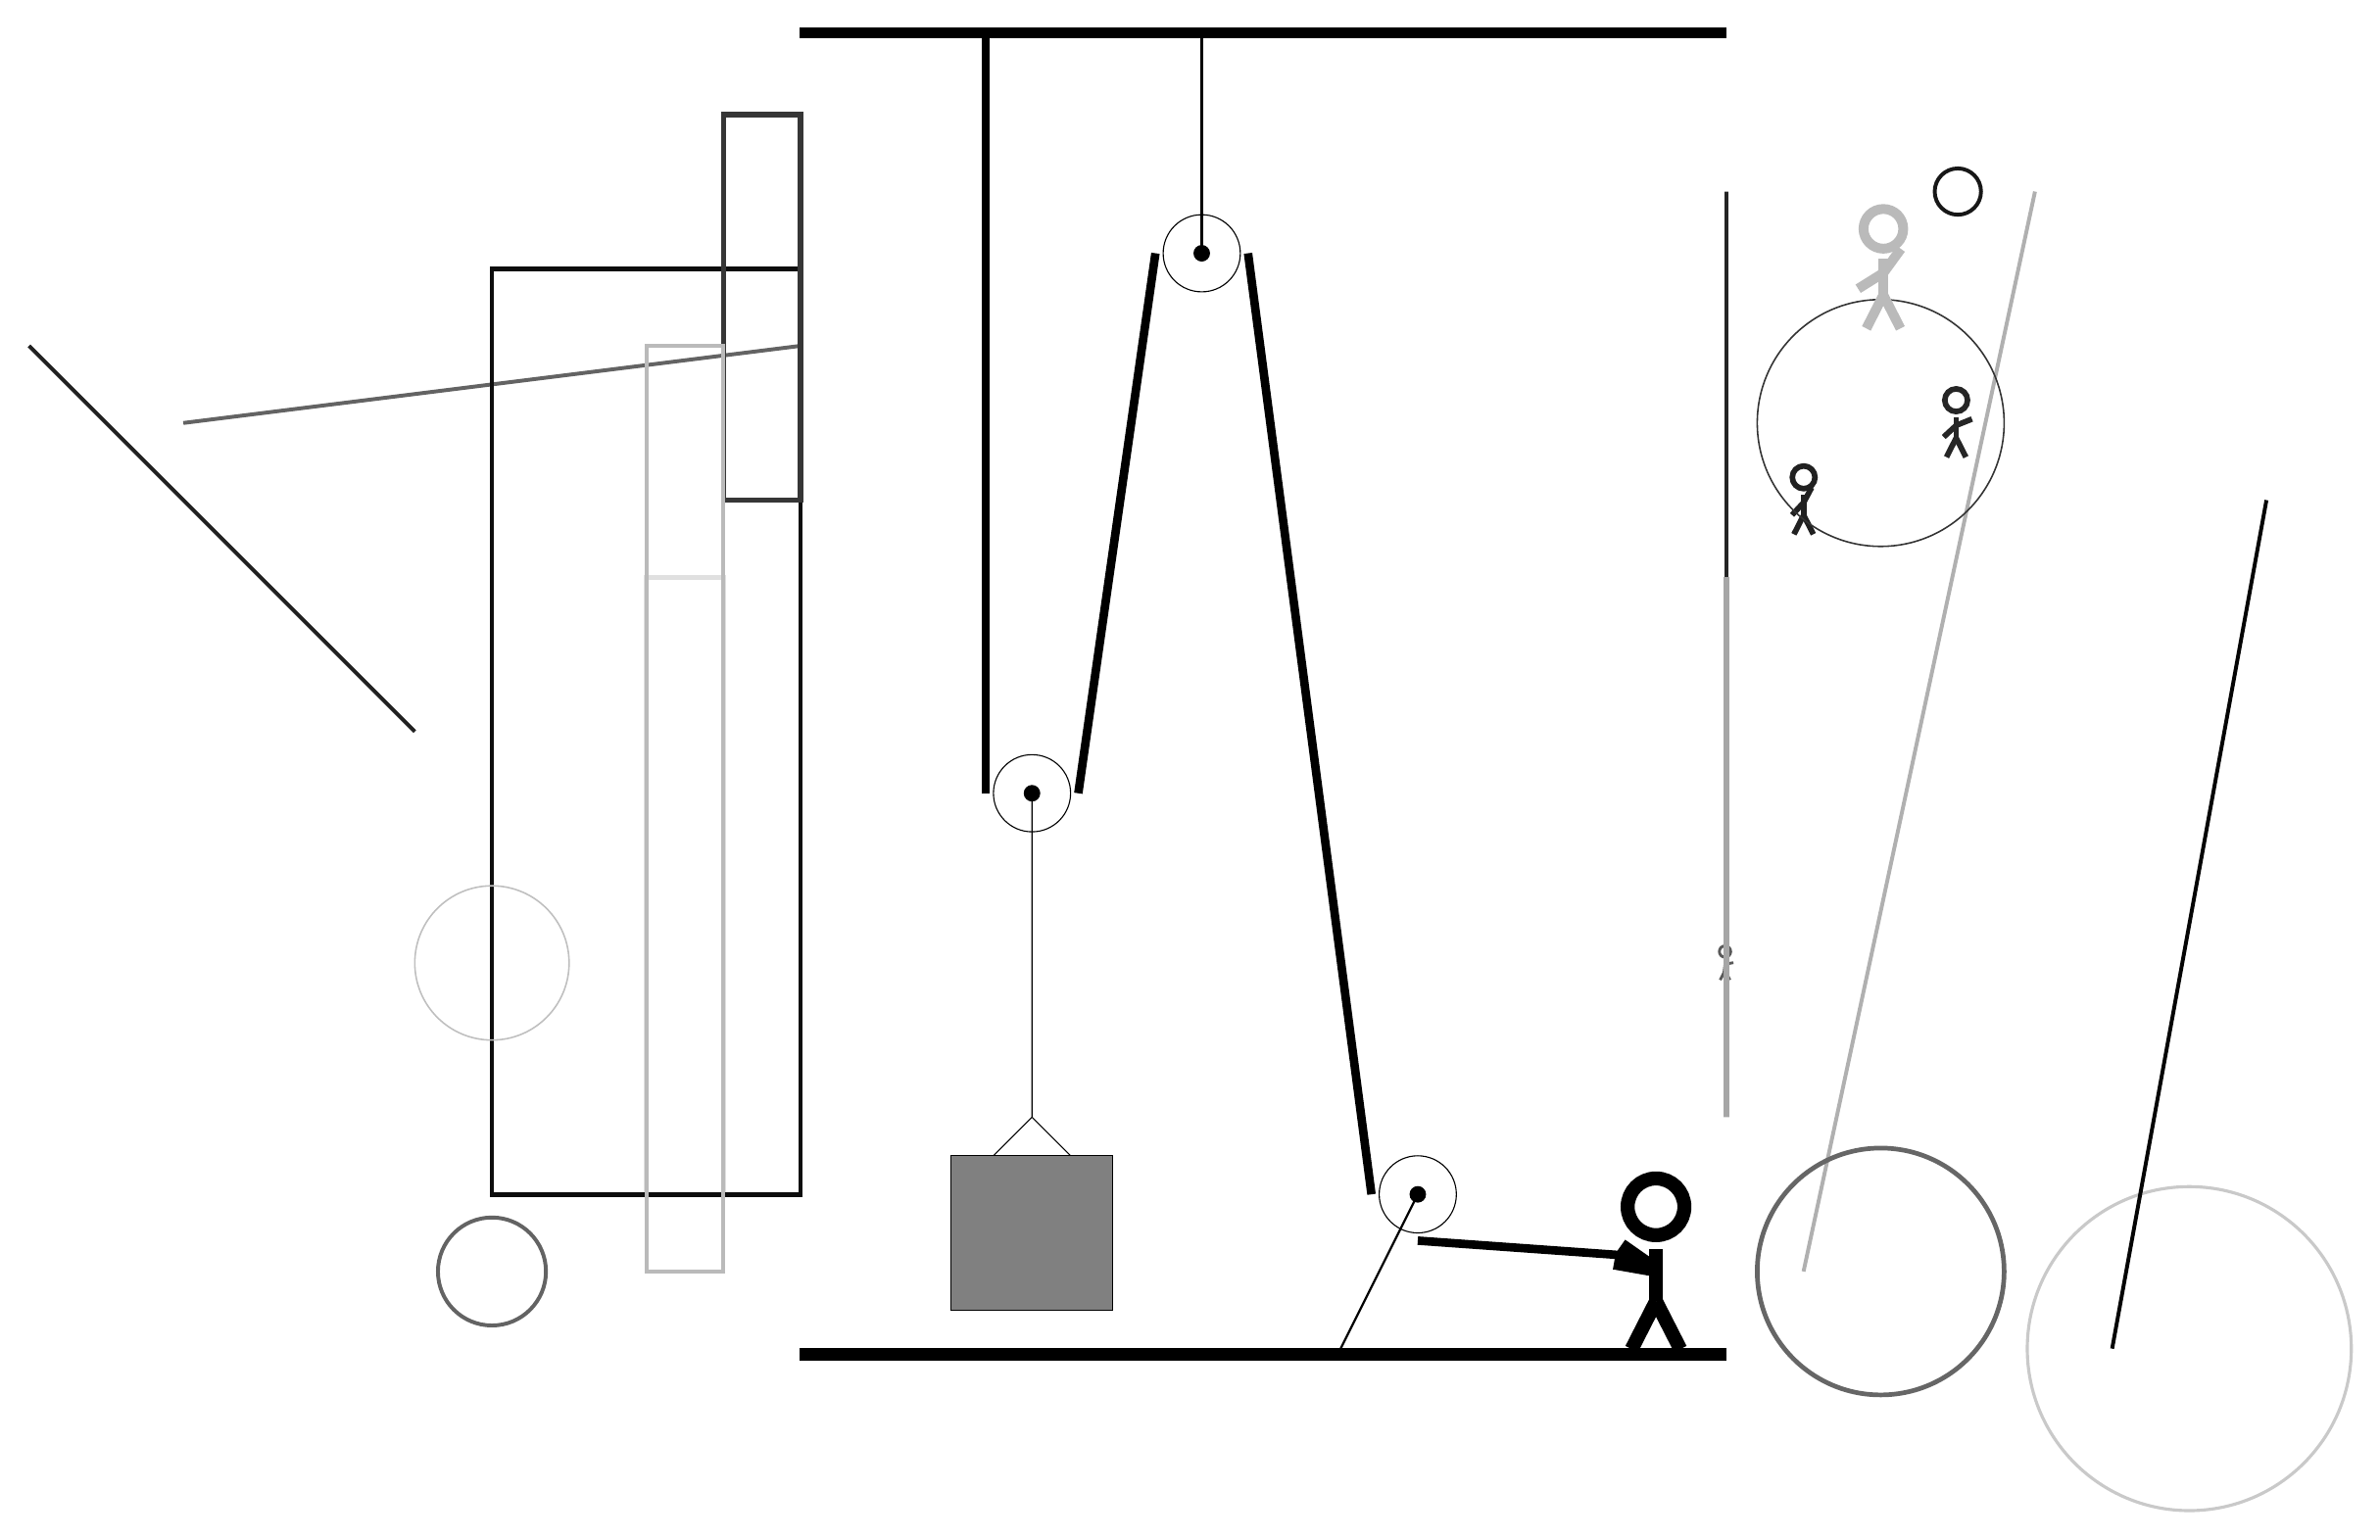
\begin{tikzpicture}
			%%%%% START %%%%%
			
			\draw[fill=black] (-2, 14) rectangle (10, 14.125);
			
			\draw (3.2, 11.2) circle (0.5);
			\draw[fill=black] (3.2, 11.2) circle (0.1);
			\draw[thick] (3.2, 11.2) -- (3.2, 14);
			
			\draw (6, -1) circle (0.5);
			\draw[fill=black] (6, -1) circle (0.1);
			\draw[thick] (6, -1) -- (5, -3);
			
			\draw (1, 4.2) circle (0.5);
			\draw[fill=black] (1, 4.2) circle (0.1);
			
			\draw[line width=0.5mm, color=black!31](11, -2) -- (14, 12);
			
			\draw [line width=0.5mm, color=black!61](-6, -2) circle (0.7);
			\draw[line width=0.5mm, color=black!61](-2, 10) -- (-10, 9);
			\draw[line width=0.5mm, color=black!88](10, 5) -- (10, 3);
			
			\draw [line width=0.5mm, color=black!91](13, 12) circle (0.3);
			
			\draw[line width=0.6mm, color=black!12] (-3, 7) rectangle (-4, -1);
			\draw [line width=0.4mm, color=black!21](16, -3) circle (2.1);
			\draw [line width=0.6mm, color=black!60](12, -2) circle (1.6);
			\draw[line width=0.5mm, color=black!98](15, -3) -- (17, 8);
			\draw[line width=0.5mm, color=black!86] (10, 7) rectangle (10, 12);
			\draw[line width=0.6mm, color=black!95] (-2, 11) rectangle (-6, -1);
			\node[line width=0.7mm, color=black!85] at (13, 9) {\Strichmaxerl[4][43][22]};
			\node[line width=0.6mm, color=black!65] at (10, 2) {\Strichmaxerl[2][83][10]};
			\node[line width=0.6mm, color=black!87] at (11, 8) {\Strichmaxerl[4][47][62]};
			\draw [line width=0.2mm, color=black!80](12, 9) circle (1.6);
			\draw[line width=0.5mm, color=black!87](-7, 5) -- (-12, 10);
			
			\node[line width=0.6mm, color=black!27] at (12, 11) {\Strichmaxerl[7][32][54]};
			\draw[line width=0.7mm, color=black!35] (10, 7) rectangle (10, 0);
			\draw [line width=0.2mm, color=black!25](-6, 2) circle (1.0);
			\draw[line width=0.7mm, color=black!79] (-3, 13) rectangle (-2, 8);
			\draw[line width=0.5mm, color=black!27] (-3, 10) rectangle (-4, -2);
			
			\draw (1, 4.2) -- (1, 0) -- (0.5, -0.5);
			\draw (1, 0) -- (1.5, -0.5);
			\draw[fill=black!50] (-0.05, -0.5) rectangle (2.05, -2.5);
			
			\draw[line width=1.1mm] (0.4, 14) -- (0.4, 4.2);
			\centerarc[line width=1.1mm](1, 4.2)(180:360:0.6);
			\draw[line width=1.1mm](1.6, 4.2) -- (2.6, 11.2);
			\centerarc[line width=1.1mm](3.2, 11.2)(0:180:0.6);
			\draw[line width=1.1mm](3.8, 11.2) -- (5.4, -1);
			\centerarc[line width=1.1mm](6, -1)(180:270:0.6);
			\draw[line width=1.1mm](6, -1.6) -- (8.8, -1.8);
			
			\node at (9, -1.9) {\Strichmaxerl[10][-35][170]};
			
			\draw[fill=black] (-2, -3) rectangle (10, -3.15);
			
			%%%%% END %%%%%
		\end{tikzpicture}
	\end{figure}	
\end{document}